\section{Orientation}
\label{sec:exp_orient}

\begin{figure*}[!tb]\centering
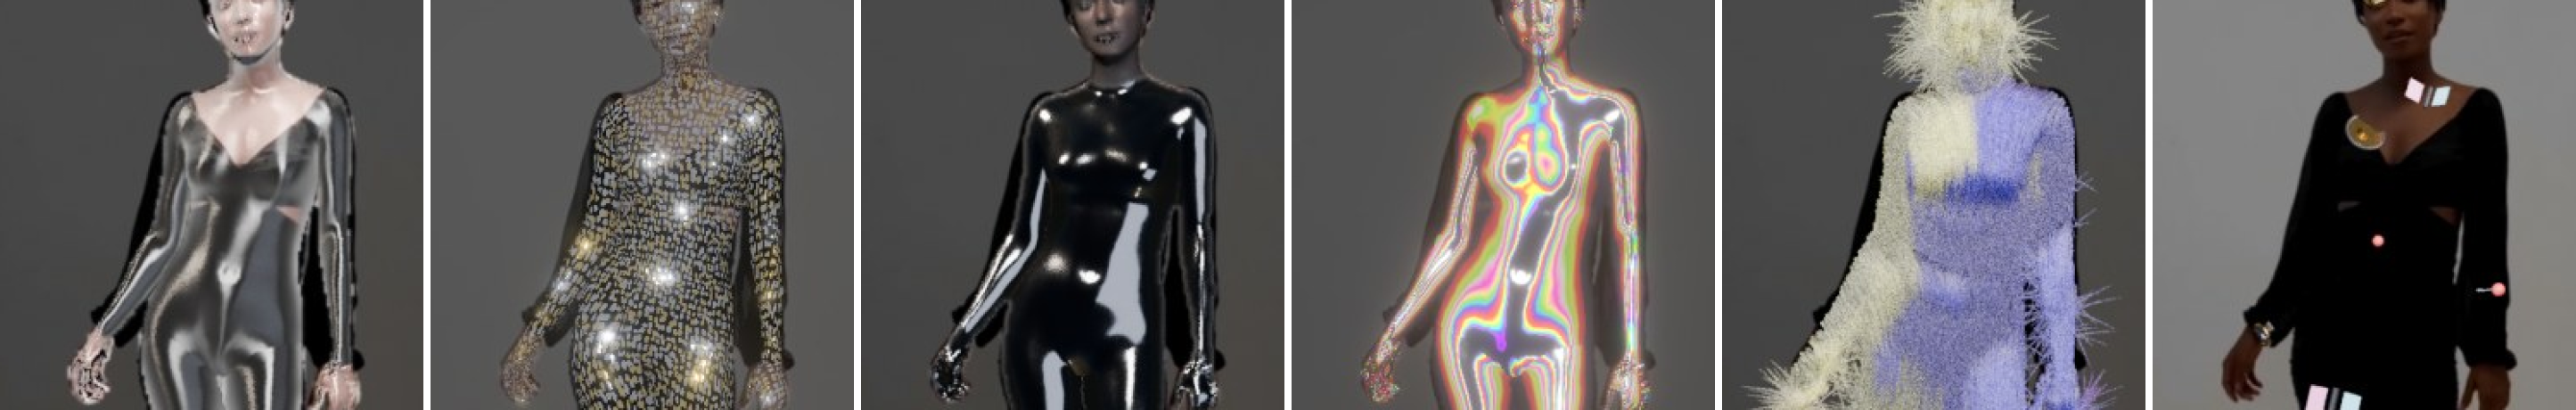
\includegraphics[width=0.94\linewidth]{figs/fig_framefield.png}
\caption{\textbf{The frame field, used forward} on real video: \textbf{(a)} anisotropic satin, a
Kajiya--Kay~\cite{kajiya1989rendering} lobe whose axis is the predicted tangent --- the one effect
a normal map cannot produce; \textbf{(b)} sequins on canonical UV cells, welded to skin not image;
\textbf{(c)} chrome, a readout of the predicted normals; \textbf{(d)} a Stam
grating~\cite{stam1999diffraction} painting twist as colour; \textbf{(e)} Cycles fur along the
unprojected 3D tangent; \textbf{(f)} orientation-locked object attachment. Qualitative: no
orientation ground truth exists for these frames.}
\label{fig:framefield}
\end{figure*}

On BEDLAM-val the shipped models reach $6.77^\circ$ (\texttt{dp\_csc\_C}) and $6.86^\circ$ (W-M)
mean geodesic error under the end-to-end readout, against $6.98^\circ$ for W-B (\cref{tab:coco});
the number is stable across the data and recipe changes of \cref{sec:exp_csc} on this clean split,
and the entire gap opened by occlusion data appears not here but on held-out interaction sequences
($14.80^\circ\!\rightarrow\!6.89^\circ$). What the field buys is qualitative
(\cref{fig:framefield}): each render is a \emph{pullback} of the prediction, so nothing inverts it,
tracks a point, fits a mesh or filters temporally.

\paragraph{We have no baseline for this number, and that is the main weakness of the orientation
result.} $6.77^\circ$ is measured against our own checkpoints only. Three comparisons would make it
interpretable and we ran none: fitting a body model per image and rendering its frame
field~\cite{zhu2024champ}; differentiating the predicted $(u,v)$ map, pushing the Jacobian through
the template and orthonormalising --- a frame with no extra head and no extra supervision, the
obvious null hypothesis for our contribution; and an off-the-shelf normal
estimator~\cite{bae2024dsine,khirodkar2024sapiens} plus a template tangent for the twist. Until at
least the second is run, the paper establishes that a per-pixel $SO(3)$ output can be trained to
this accuracy at this cost, not that an explicit rotation head is the best way to obtain one.

A ladder of one-change-at-a-time runs in one from-scratch lineage (supp., under an \emph{oracle}
gather not comparable with the numbers above) takes the geodesic error from $9.01^\circ$ to
$7.30^\circ$: a per-part rather than shared rotation head is worth $-0.53^\circ$, layer-wise decay
$-0.43^\circ$, a longer schedule the rest. Its last rungs lie on the $10^{-3}$ branch, the
synthetic optimum that costs $3.4$ COCO AP points, so we do not ship it and never evaluated the
shipped branch's $120$k endpoint under that readout; and being oracle-gathered it does not charge
the per-part design the $0.65^\circ$ gather penalty a shared head would not pay at all --- we never
ran the shared head end to end, so its net deployment effect is unmeasured while its COCO cost,
$1.8$ AP points, is measured. The field is not capped by correspondence quality: CSC improves
correspondence substantially at fixed rotation supervision, yet geo\_e2e moves only within
$6.77$--$6.90^\circ$, and the identifiable term is the gather --- the $24$ charts are disjoint, so
a misclassified pixel reads a wrong chart --- which puts the next lever on the part head.
% [log] rungs: jobs 5369862 / 5390804 / 5390877 / 5390900 (58k); chain 5403066-68 (@120k).
